\documentclass[a4paper]{article}

%use the english line for english reports
%usepackage[english]{babel}
\usepackage[portuguese]{babel}
\usepackage[utf8]{inputenc}
\usepackage{indentfirst}
\usepackage{graphicx}
\usepackage{verbatim}
\usepackage{fancyhdr}
\usepackage{listings}
\usepackage{color}

\definecolor{dkgreen}{rgb}{0,0.6,0}
\definecolor{gray}{rgb}{0.5,0.5,0.5}
\definecolor{mauve}{rgb}{0.58,0,0.82}

\lstset{frame=tb,
  language=Prolog,
  aboveskip=3mm,
  belowskip=3mm,
  showstringspaces=false,
  columns=flexible,
  basicstyle={\small\ttfamily},
  numbers=none,
  numberstyle=\tiny\color{gray},
  keywordstyle=\color{blue},
  commentstyle=\color{dkgreen},
  stringstyle=\color{mauve},
  breaklines=true,
  breakatwhitespace=true,
  tabsize=3
  }

\begin{document}


\setlength{\textwidth}{16cm}
\setlength{\textheight}{22cm}

\title{\Huge\textbf{FABRIK}\linebreak\linebreak\linebreak
\Large\textbf{Relatório Final}\linebreak\linebreak
\linebreak\linebreak

\includegraphics[scale=0.1]{images/feup-logo.png}\linebreak\linebreak
\linebreak\linebreak
\Large{Mestrado Integrado em Engenharia Informática e Computação} \linebreak\linebreak
\Large{Programação em Lógica}\linebreak
}

\author{\textbf{Grupo Fabrik3:}\\
\linebreak\\
André Cruz - 201503776 \\
Edgar Carneiro - 201503748 \\
\linebreak\linebreak \\
 \\ Faculdade de Engenharia da Universidade do Porto \\ Rua Roberto Frias, s\/n, 4200-465 Porto, Portugal \linebreak\linebreak\linebreak
\linebreak\linebreak\vspace{1cm}}

\maketitle
\thispagestyle{empty}

%************************************************************************************************
%************************************************************************************************

\newpage

\section*{Resumo}

Este trabalho tem como objetivo a modelação e implementação do jogo de tabuleiro \textit{Fabrik}, com uma representação na linha de comandos, assim como os modos de jogo \textit{jogador vs jogador}, \textit{jogador vs computador} e \textit{computador vs computador}. Tratando-se de um jogo de tabuleiro, foi necessário decidir um modelo apropriado para representar o estado do jogo, desenvolver predicados para verificar se determinada jogada é válida, e predicados para determinar quando o jogo termina. Foi também necessário implementar resilientes mecanismos de obtenção de \textit{input} do utilizador, e menus para interface com o utilizador.

Relativamente à escolha automática de uma jogada por parte do computador, esta tem dois níveis: um mais fácil, em que a jogada é escolhida aleatóriamente; e um mais difícil, em que é identificada a melhor jogada que é possível efetuar tendo em conta o ocntexto atual (algoritmo ganancioso). Neste sentido, desenvolvemos vários predicados para a avaliação quantitativa de uma jogada e do estado do jogo, tendo sido alcançados os nossos objetivos de dificuldade de jogo contra o computador.

Recorrendo à excelente bibliografia indicada pelo professores, \cite{sterling_shapiro_warren_2010} e \cite{carlsson_fruhwirth_2016}, foi possível resolver todos os problemas que encontramos na implementação deste jogo, bem como uma aprendizagem contínua dos conceitos relacionados com este paradigma de programação.

Para finalizar, achamos que o trabalho apresentado representa uma eficiente, completa e compreensiva modelação do jogo \textit{Fabrik} e dos seus conceitos, e temos orgulho no resultado final.

\newpage

\tableofcontents

%************************************************************************************************
%************************************************************************************************

%*************************************************************************************************
%************************************************************************************************

\newpage

%%%%%%%%%%%%%%%%%%%%%%%%%%
\section{Introdução}

Este trabalho foi desenvolvido no âmbito da unidade curricular de Programação em Lógica, integrada no 3º ano do Mestrado Integrado em Engenharia Informática e Computação, tendo como objetivo aprofundar os conhecimentos adquiridos nas aulas teóricas e práticas desta unidade curricular, bem como a abordagem de problemas mais práticos com recurso à linguagem \textit{PROLOG}. Deste modo, propusemo-nos a implementar e modelar do jogo de tabuleiro \textit{Fabrik}, sendo possível os modos de jogo \textit{jogador vs jogador}, \textit{jogador vs computador} e \textit{computador vs computador} (com dois níveis de dificuldade).

A escolha deste jogo, que foi selecionado dentro de um leque de opções disponibilizadas pelos docentes, prendeu-se no conjunto de conceitos intuitivos que incorpora (\textit{e.g.} linhas de visão das peças), permitindo uma rápida aprendizagem das regras, assim como um desafio na implementação de restrições de jogadas e avaliação do tabuleiro. Esta aparente simplicidade é no entanto contrabalançada com o facto de cada jogada ter dois passos: a colocação do \textit{worker}, e a colocação de uma peça \textit{black}/\textit{white} (estando este segundo passo fortemente constrangido pelo primeiro).

Este relatório está dividido em várias secções, sendo a presente a primeira:
\begin{enumerate}
\item Na segunda secção deste relatório, é feita uma pequena introdução à história do jogo \textit{Fabrik}, aos componentes físicos necessários para jogar, e às regras oficiais do jogo;
\item Na secção seguinte, são apresentados vários detalhes da nossa implementação, desde a representação visual do tabuleiro ao algoritmo de cálculo da melhor jogada possível dado um determinado estado de jogo;
\item Na quarta secção, é descrita a interface com o utilizador, que consiste nos menus e input esperado em cada um destes;
\item Na última secção, são tecidas conclusões acerca do desenvolvimento deste trabalho e do seu enquadramento curricular.
\end{enumerate}

\newpage

%%%%%%%%%%%%%%%%%%%%%%%%%%
\section{O Jogo \textit{Fabrik}}

\subsection{História}
O jogo - \textit{Fabrik} - foi recentemente desenvolvido por Dieter Stein, em Agosto de 2017, como parte de um estudo para o desenvolvimento de um novo jogo, Urbino.

\subsection{Material}
\begin{itemize}
	\item Tabuleiro quadrangular
	\item Quantidade suficiente de peças pretas e brancas
	\item Duas peças vermelhas chamadas trabalhadores
\end{itemize}

\begin{figure}[h!]
\begin{center}

\includegraphics[height=3cm,width=3cm]{images/fabrik_empty_board.png}
\caption{Tabuleiro vazio de 11 x 11 espaços}
\label{Figura 1}
\end{center}
\end{figure}

\subsection{Regras}
A implementação deste jogo foi baseada no manual de regras oficiais \cite{games_and_puzzles_by_dieter_stein}.

As pretas (jogador que joga com peças de cor preta) começam por colocar um dos trabalhadores num espaço à sua escolha. De seguida, as brancas (jogador que joga com peças de cor branca) colocam o outro trabalhador num espaço livre. De seguida, as pretas decidem quem começa por jogar.

O jogo procede por turnos, sendo que em cada turno um jogador pode, se assim optar, mover um dos trabalhadores para um espaço vazio. De seguida, o jogador deve jogar colocar uma das suas peças num ponto de interseção entre as “linhas de visão dos dois trabalhadores”. As linhas de visão dos trabalhadores são as linhas na diagonal, horizontal e vertical sobre as quais os trabalhadores se encontram posicionados.

\begin{figure}[h!]
\begin{center}
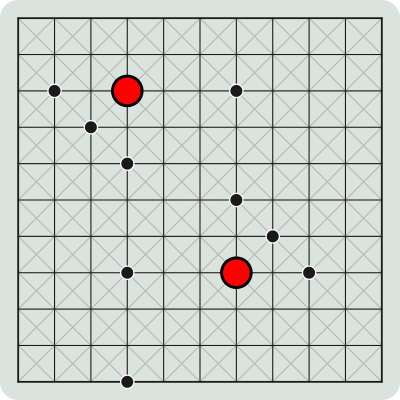
\includegraphics[height=3cm,width=3cm]{images/fabrik_intersection.png}
\caption{Pontos de interseção entre os dois trabalhadores}
\label{Figura 2}
\end{center}
\end{figure}

No caso especial em que os dois trabalhadores se encontram sobre uma mesma linha ortogonal ou diagonal, apenas os espaços entre eles são considerados pontos de interseção (se estiverem vazios), ao invés da totalidade dessa linha.

Ganha o jogo o jogador que consiga criar uma linha de pelo menos 5 pedras da sua cor, ortogonalmente ou diagonalmente. Um jogador ganha também o jogo se o seu adversário não conseguir posicionar nenhum dos trabalhadores de forma a poder colocar uma pedra sua no tabuleiro.

\begin{figure}[h!]
\begin{center}
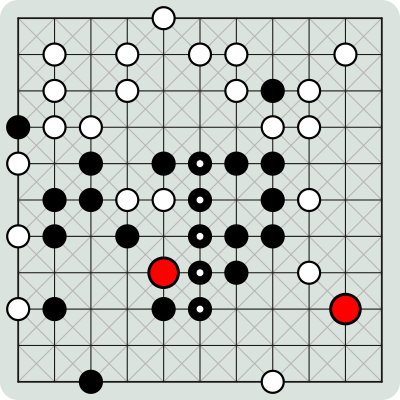
\includegraphics[height=3cm,width=3cm]{images/fabrik_full_board.png}
\caption{Final de uma partida de Fabrik, com vitórias das pretas}
\label{Figura 3}
\end{center}
\end{figure}

\vfill
\textbf{Referências:}\newline
https://spielstein.com/games/fabrik\newline
https://spielstein.com/games/fabrik/rules

\newpage

%%%%%%%%%%%%%%%%%%%%%%%%%%
\section{Lógica do Jogo}

Descrever o projeto e implementação da lógica do jogo em Prolog, incluindo a forma de representação do estado do tabuleiro e sua visualização, execução de movimentos, verificação do cumprimento das regras do jogo, determinação do final do jogo e cálculo das jogadas a realizar pelo computador utilizando diversos níveis de jogo. Sugere-se a estruturação desta secção da seguinte forma:

\subsection{Representação do Estado do Jogo}

A representação dos estados de jogo é feita com recurso a uma lista de listas, de forma a simular o uso de uma Matriz. Seguem de seguida, a representaçao de diferentes estados de jogo:\newline



Representação do \textbf{estado inicial}:

\begin{small}
\begin{lstlisting}
[[none, none, none, none,  none, none,  none, none, none, none, none],
 [none, none, none, none,  none, none,  none, none, none, none, none],
 [none, none, none, none,  none, none,  none, none, none, none, none],
 [none, none, none, none,  none, none,  none, none, none, none, none],
 [none, none, none, none,  none, none,  none, none, none, none, none],
 [none, none, none, none,  none, none,  none, none, none, none, none],
 [none, none, none, none,  none, none,  none, none, none, none, none],
 [none, none, none, none,  none, none,  none, none, none, none, none],
 [none, none, none, none,  none, none,  none, none, none, none, none],
 [none, none, none, none,  none, none,  none, none, none, none, none],
 [none, none, none, none,  none, none,  none, none, none, none, none]]
\end{lstlisting}
\end{small}

\begin{figure}[h!]
\centering
\begin{minipage}{.35\textwidth}
	\centering
	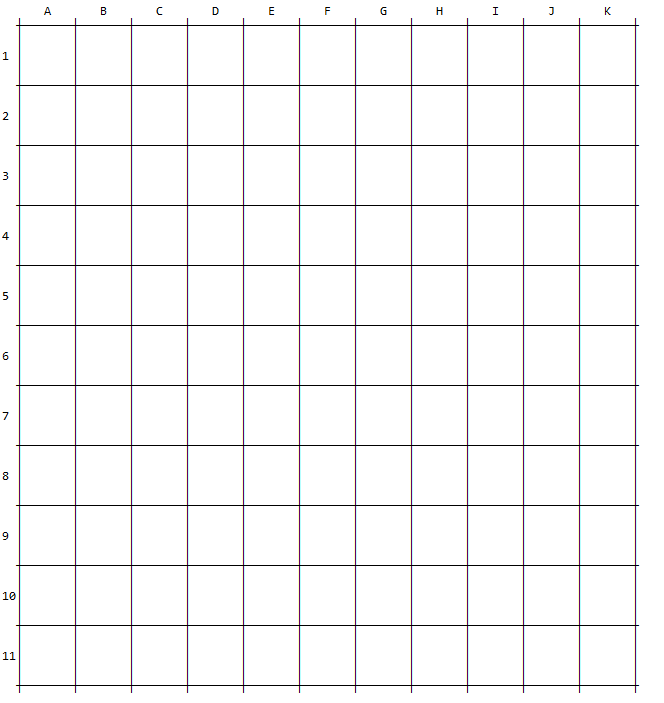
\includegraphics[width=\textwidth]{images/self_empty_board.png}
	\caption{Representação do estado inicial na consola}
	\label{Figura 4}
\end{minipage}
\quad \quad
\begin{minipage}{.35\textwidth}
	\centering
	
\includegraphics[width=\textwidth]{images/fabrik_empty_board.png}
	\caption{Tabuleiro original Vazio}
	\label{Figura 5}
\end{minipage}
\end{figure}

\clearpage

Representação de um possível \textbf{estado intermédio}:\newline

\begin{small}
\begin{lstlisting}
[[ none, none, none, none, none, none, none, none, none, none, none],
 [ none, none, none, none, none, white, worker, none, none, none, none],
 [ none, none, none, none, none, none, white, black, white, none, none],
 [ none, white, white, none, none, none, none, white, white, none, none],
 [white, none, none, none, black, black, none, black, none, none, none],
 [ none, none, black, white, none, none, none, none, white, none, none],
 [ none, black, none, none, none, black, black, black, none, none, none],
 [ none, none, none, none, none, none, black, none, white, none, none],
 [ none, none, none, none, none, black, none, none, none, none, none],
 [ none, none, none, none, worker, none, none, none, none, none, none],
 [ none, none, none, none, none, none, none, none, none, none, none]]
\end{lstlisting}
\end{small}

\begin{figure}[h!]
\begin{center}
	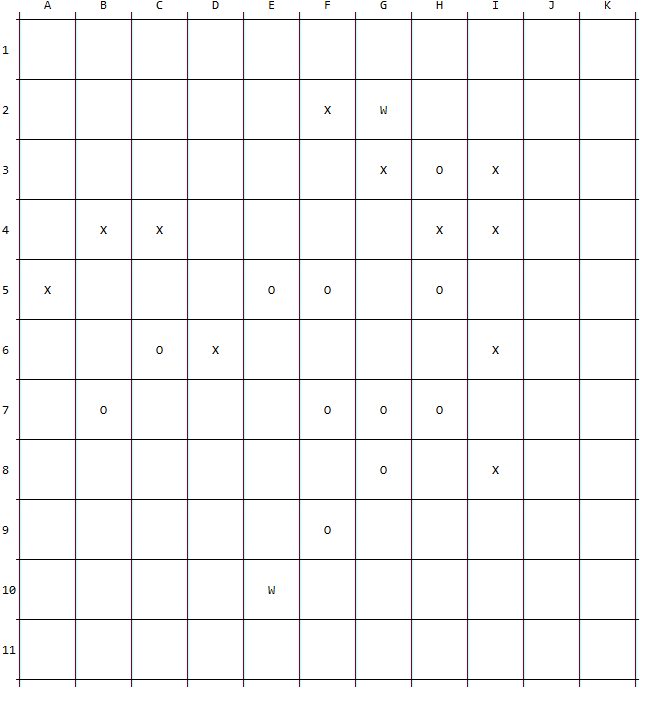
\includegraphics[height=6cm, width=6cm]{images/self_semi_board.png}
	\caption{Representação na consola, de um possível estado intermédio}
	\label{Figura 6}
\end{center}
\end{figure}

\clearpage
Representação de um possível \textbf{estado final}:\newline

\begin{small}
\begin{lstlisting}
[[ none, none, none, none, white, none, none, none, none, none, none],
 [ none, white, none, white, none, white, white, none, none,white, none],
 [ none, white, none, white, none, none,white, black, white, none, none],
 [black, white, white, none, none, none, none, white, white, none, none],
 [white, none, black, none,black, black, black, black, none, none, none],
 [none, black, black, white,white, black, none, black,white, none, none],
 [white, black, none,black, none, black, black, black, none, none, none],
 [ none, none, none, none, worker, black, black, none,white, none, none],
 [white, black, none, none,black, black, none, none, none, worker, none],
 [ none, none, none, none, none, none, none, none, none, none, none],
 [ none, none, black, none, none, none, none, white, none, none, none]]
\end{lstlisting}
\end{small}

\begin{figure}[h!]
\centering
\begin{minipage}{.35\textwidth}
	\centering
	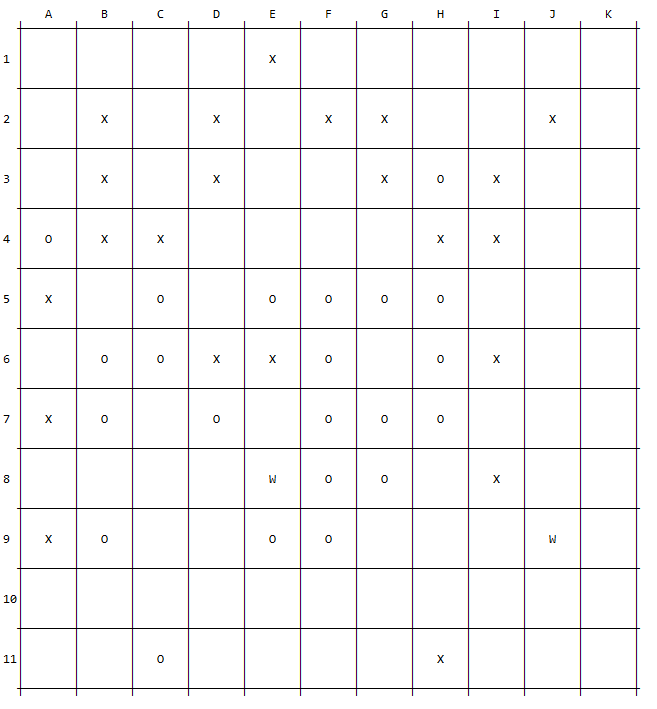
\includegraphics[width=\textwidth]{images/self_full_board.png}
	\caption{Representação do estado final na consola}
	\label{Figura 7}
\end{minipage}
\quad \quad
\begin{minipage}{.35\textwidth}
	\centering
	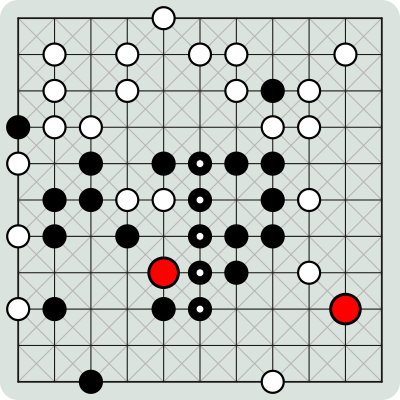
\includegraphics[width=\textwidth]{images/fabrik_full_board.png}
	\caption{Representção do mesmo estado final, no tabuleiro original}
	\label{Figura 8}
\end{minipage}
\end{figure}

\clearpage


%%%%%%%%%%%%%%%%%%%%%%%%%%
\subsection{Visualização do Tabuleiro}

Para a representação do tabuleiro em modo de texto, foi criado o seguinte código em prolog:
\begin{lstlisting}[language=prolog]
% Dictionary for Board Elements
translate(none, 32). %Empty Cell
translate(black, 79). %Dark Pieces
translate(white, 88). %White Pieces
translate(worker, 9608). %Red Workers

(...)

% General PrintBoard
printBoard(Board):-
        boardSize(N),
        printBoard(Board, N), !.

% Board Printing - arguments: Board and Board size
printBoard(Board, N):-
        clearConsole,
        write('  '), printHorizontalLabel(N, N),
        printBoard(Board, N, 1), !.

printBoard([], N, _):-
        printRowDivider(N), nl.

printBoard([Line | Board], N, CurrentL):-
        printRowDivider(N),
        printDesignRow(N),
        printVerticalLabel(CurrentL),
        put_code(9474),
        printLine(Line),
        printDesignRow(N),
        NewL is (CurrentL + 1),
        printBoard(Board, N, NewL).

printLine([]):- nl.
printLine([Head | Tail]) :-
        translate(Head, Code),
        write('   '),
        put_code(Code),
        write('   '), put_code(9474),
        printLine(Tail).

%  AESTHETICS

printRowDivider(N):-
        write('  '),
        put_code(9532),
        printRowDividerRec(N).

printRowDividerRec(0) :- nl.
printRowDividerRec(N) :-
        put_code(9472), put_code(9472), put_code(9472), put_code(9472),
        put_code(9472), put_code(9472), put_code(9472), put_code(9532),
        N1 is (N-1),
        printRowDividerRec(N1).

printDesignRow(N):-
        write('  '),
        put_code(9474),
        printDesignRowRec(N).

printDesignRowRec(0) :- nl.
printDesignRowRec(N) :-
        write('       '), put_code(9474),
        N1 is (N-1),
        printDesignRowRec(N1).

%Dictionary for Labels
getLabel( 0, 'A').
getLabel( 1, 'B').
getLabel( 2, 'C').
getLabel( 3, 'D').
getLabel( 4, 'E').
getLabel( 5, 'F').
getLabel( 6, 'G').
getLabel( 7, 'H').
getLabel( 8, 'I').
getLabel( 9, 'J').
getLabel(10, 'K').
getLabel(11, 'L').
getLabel(_,_):-
        write('Error: Unrecognized Label.'), nl,
        fail.

printHorizontalLabel(0, _):- nl.
printHorizontalLabel(N, Total):-
        Pos is (Total-N),
        getLabel(Pos, L),
        write('    '), write(L), write('   '),
        N1 is (N-1),
        printHorizontalLabel(N1, Total).        

printVerticalLabel(CurrentL):-
        CurrentL < 10,
        write(CurrentL),
        write(' ').

printVerticalLabel(CurrentL):-
        write(CurrentL).

\end{lstlisting}

Representação de um tabuleiro, usando o código mencionado:\newline

\begin{figure}[h!]
\begin{center}
	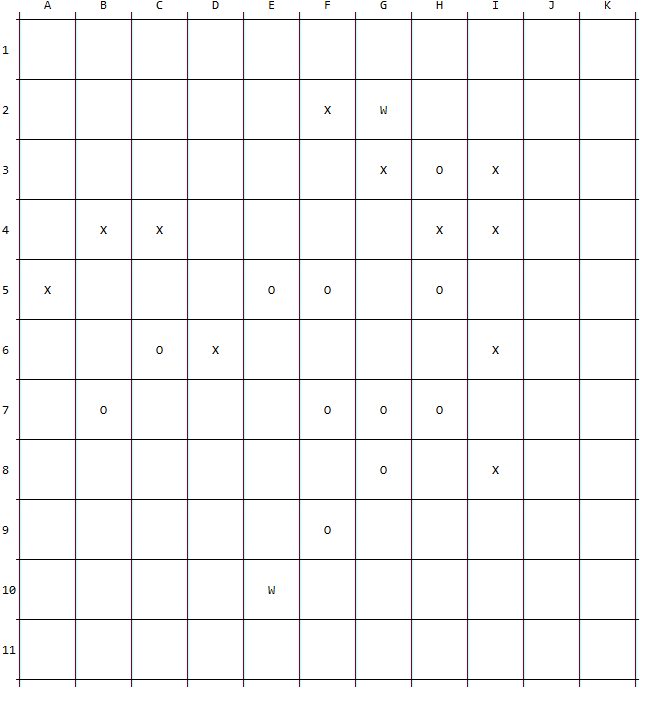
\includegraphics[height=4cm, width=4cm]{images/self_semi_board.png}
	\caption{Representação de um tabuleiro na consola}
	\label{Figura 9}
\end{center}
\end{figure}

\newpage

\subsection{Lista de Jogadas Válidas} Obtenção de uma lista de jogadas possíveis. Exemplo: \textit{valid\_moves(+Board, -ListOfMoves)}.

\newpage

\subsection{Execução de Jogadas} Validação e execução de uma jogada num tabuleiro, obtendo o novo estado do jogo. Exemplo: \textit{move(+Move, +Board, -NewBoard)}.

\newpage

\subsection{Avaliação do Tabuleiro} Avaliação do estado do jogo, que permitirá comparar a aplicação das diversas jogadas disponíveis. Exemplo: \textit{value(+Board, +Player, -Value)}.

\newpage

\subsection{Final do Jogo} Verificação do fim do jogo, com identificação do vencedor. Exemplo: \textit{game\_over(+Board, -Winner)}.

\newpage

\subsection{Jogada do Computador} Escolha da jogada a efetuar pelo computador, dependendo do nível de dificuldade. Por exemplo: \textit{choose\_move(+Level, +Board, -Move)}.

\newpage

%%%%%%%%%%%%%%%%%%%%%%%%%%
\section{Interface com o Utilizador}

Descrever o módulo de interface com o utilizador em modo de texto.

\newpage

%%%%%%%%%%%%%%%%%%%%%%%%%%
\section{Conclusões}
Que conclui deste projecto? Como poderia melhorar o trabalho desenvolvido?


\clearpage
\addcontentsline{toc}{section}{Bibliografia}
\renewcommand\refname{Bibliografia}
\bibliography{myrefs}
\bibliographystyle{ieeetr}


\newpage
\appendix
\section{Nome do Anexo}
Código Prolog implementado devidamente comentado e outros elementos úteis que não sejam essenciais ao relatório.

\end{document}
